\chapter{Variational InfoNCE}

\section{Motivations}
%\section{Problem setting}
	In the previous section we discussed two categories of representation learning though deep learning. First, we discussed the autoencoder and its variational counterpart, which minimise the reconstruction error. Secondly, we discussed Contrastive Predictive Coding and Greedy InfoMax, both of which optimise the Info NCE objective. This approach seeks to maximise the mutual information between the encodings of data patches that are temporally nearby. The latent representations obtained from all four methods can then be utilised for downstream tasks \cite{bengioRepresentationLearningReview2013, weiRecentAdvancesVariational2021, oordRepresentationLearningContrastive2019, lowePuttingEndEndtoEnd2020}
	
	% repr learn autoenc + vae (disentenglement)
		The autoencoder's sole objective is to define representations which allow to reconstruct the original data. As a result, the representations may serve well for data compression, however, no additional constraints are enforced, such as feature disentanglement and thus the latent space may still be hard to work with for downstream tasks \cite{tschannenRecentAdvancesAutoencoderBased2018}. Meanwhile, VAEs' additional regularisation term, results in representations which break down or disentangle each feature into a narrowly defined variable and encodes them as separate dimensions \cite{weiRecentAdvancesVariational2021}. This additional constrained may result in better suited representations for downstream tasks. % TODO: I could reformulate this, and mention meta priors such as in this paper: https://arxiv.org/pdf/1812.05069.pdf

	% cpc contrasts noise -> smaller architect
		Both autoencoders and VAEs merely learn to reconstruct the data. Hence, all the "information" that is important to reconstruct the data will be maintained in the latent representation, whether the information is useful for downstream tasks or not. Meanwhile, optimising latent representations for the InfoNCE objective will maintain shared information between temporally nearby patches, while discarding local noise. Reconstruction is thus not needed for training. This strategy has the tremendous benefit that a decoder block is not required, resulting in a significantly simplified architecture, meanwhile maintaining state-of-the-art performance \cite{stackeEvaluationContrastivePredictive2020}. A second benefit of these models is that they are directly compatible with sequential data.
		
	% lead to interpretabil
		Both categories (reconstruction and information maximisation algorithms) possess the ability to obtain useful representations for various downstream tasks. However, the content of these representations may not always be intuitive to humans and their structure may be difficult to comprehend. While CPC and GIM are considered state-of-the-art, their performance comes at a cost of having the least interpretable representations. Autoencoders maintain interpretability by using a decoder to reveal the information contained in the latent representation. The same transparency can also be achieved with VAEs. Additionally, by using a standard Gaussian as a prior and constraining the latent distributions to be similar to this prior, we can interpolate between representations and observe the effects through the decoder. VAEs can also result in disentangled features, further enhancing interpretability \cite{grossuttiDeepLearningInfrared2022}. In contrast, CPC and GIM do not contain a built in decoder mechanism, nor pose constraints on the latent space, significantly reducing interpretability.
		


\section{Towards decoupled training for probabilistic representations}
	% Our contribution
		In what follows next we introduce "Variational Greedy Infomax", maintaining the state-of-the-art performance obtained from optimising InfoNCE, while leveraging the interpretable and disentangled benefits from VAEs. This is achieved through by optimising a novel loss function, Variational InfoNCE loss, a combination of InfoNCE and the regularisation term from VAEs. Additionally, by splitting up the neural network into modules, as introduced in \cite{lowePuttingEndEndtoEnd2020}, we greedily optimise each module with its own instance with Variational InfoNCE, resulting in interpretability benefits from VAEs will also be applicable in-between modules. This is in contrast to VAEs where solely the final output representations are interpretable.		
				
	% How:
		% still maximise mutual information between zt, ztk, but predictions no longer fixed datapoints.
		% xt -> cpc model -> q( . | xt) = mui, sigmai
		
		As discussed in the section on Contrastive Predictive Coding, representations $\zt$ or $\ct$ are obtained via two functions $g_{enc}(\cdot)$ and $g_{ar}(\cdot)$, respectively, such that given a patch of sequential data $\xt$, the following holds true:
	
		\begin{align} % CPC: c, z
			g_{enc}(\xt) &= \zt \\
			g_{ar}(\z_1  \dots \zt) &= \ct
		\end{align}
		
		% split in modules
			Both $\zt$ or $\ct$ may serve as representations for downstream tasks. The encoding functions $\genc$ and $\gar$ are obtained by optimising a global loss function, $\Lnce$, end-to-end via backpropagation. 
			
			Instead, we split up $\genc$ into $M$ modules $g_{enc}^1, g_{enc}^2,~\dots,~g_{enc}^M$, and prevent gradients from flowing between modules, as introduced in \cite{lowePuttingEndEndtoEnd2020}. An additional optional $M+1$'th module $\gar$ can be appended. Each module is greedily optimised via a novel loss function, $\Lvnce$, which we will define in a following subsection.
			This is depected in figure \ref{fig:variationalgim}.
			
			
			\begin{align} % g_enc1, ...
				g_{enc}^1(\xt) &= \zt^1 \\
				g_{enc}^m(\zt^{m-1}) &= \zt^m \\
				g_{ar}(\z_t^M \dots \zt^M) &= \ct
			\end{align}
		
		\begin{figure} % fig: overview multiple modules
			\centering
			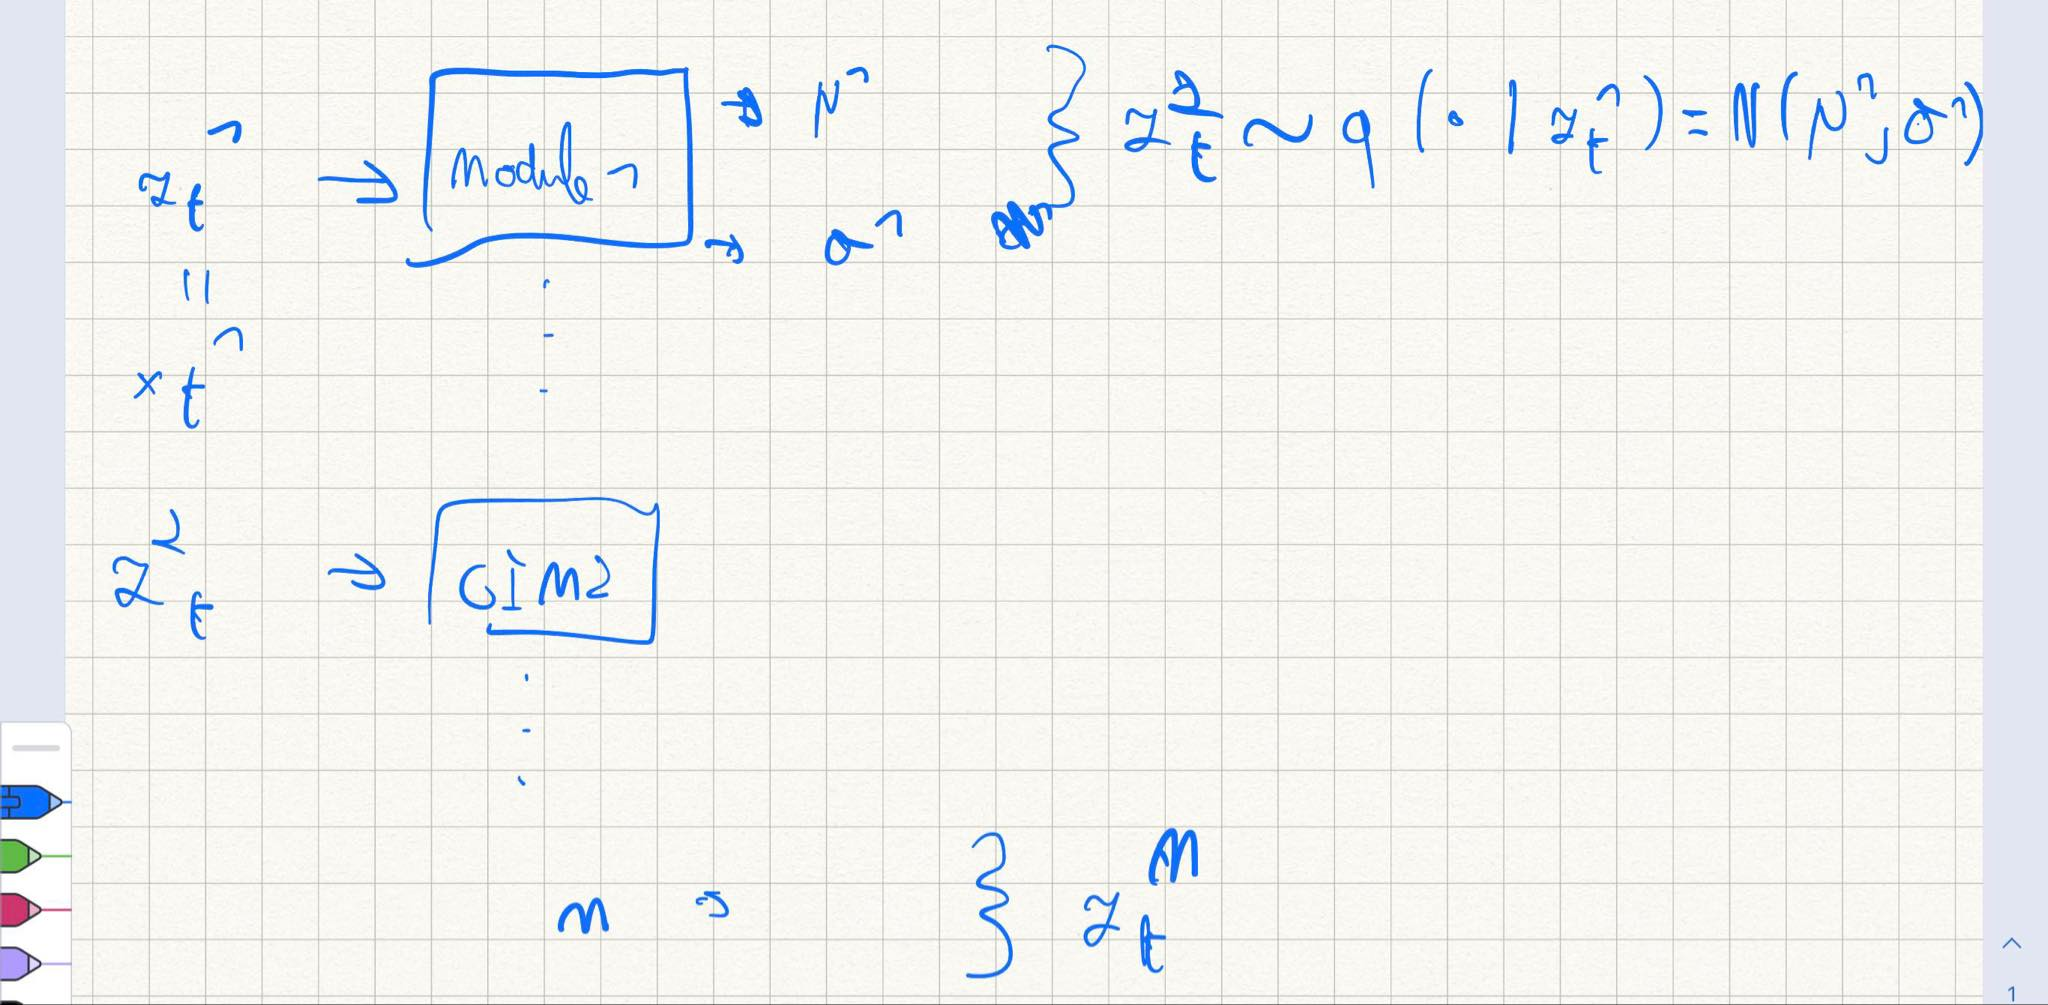
\includegraphics[width=0.7\linewidth]{temp_variational_gim}
			\caption{}
			\label{fig:variationalgim}
		\end{figure}
		
		
		% TODO: WANNEER OVER GRADIENTS BEGINT, A SINGLE MODULE IS DEFINED AS FOLLOWS.. MET F(z m-1) -> (mu, sigm)
		
		
		% Distributions
			Where $\zt^m$ and $\ct$ are in fact vector samples from a Gaussian distribution, parametrised by $\mufat = \mu(\zt^{m-1})$ and $\sigmafat = \sigma(\zt^{m-1})$, denoted as follows:
			
			\begin{align} % distributions
				\sample{\zt^m} \sampleqdot{\zt^{m-1}}
			\end{align}
	
			
		
		The outputs from $\genc$ and $\gar$ are thus samples from a distribution. This is in contrast to CPC and GIM's encodings which remain fixed depending to the input \cite{oordRepresentationLearningContrastive2019, lowePuttingEndEndtoEnd2020}. The samples obtained from the $M$'th module $\sample{\zt^M} \sampleqdot{\zt^{M-1}}$ can then be used for downstream tasks. As a result from this probabilistic approach, a single patch of data $\xt$ will correspond to multiple representations $\zt^M$. Thus, for downstream tasks with scarce labelled data, may result in the new data, potentially resolving downstream tasks ... TODO.
	 		%TODODODO
			The samples obtained from q( . | zM) can then be used for downstream tasks. A single xt will have multiple representations zM. This variance could be benefit. % The ability of VAEs to synthesize new data with more representation variance at state-of-art levels provides hope that the chronic scarcity of labeled data in the biomedical field can be resolved. \cite{weiRecentAdvancesVariational2021}
			
		\begin{figure} % img: single module
			\centering
			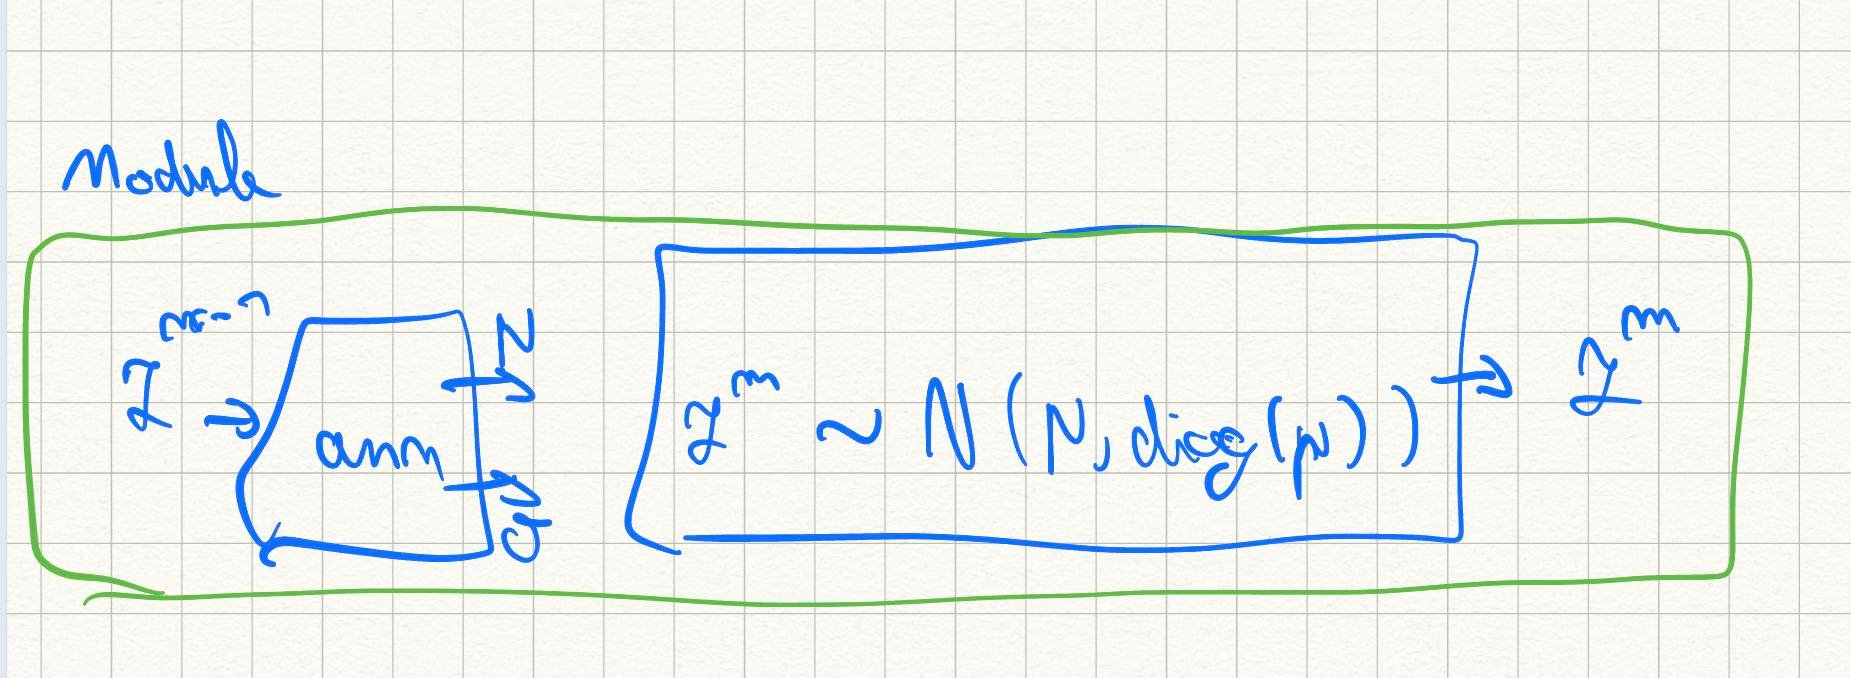
\includegraphics[width=0.7\linewidth]{temp_variational_module}
			\caption{}
			\label{fig:tempvariationalmodule}
		\end{figure}
		
		

		
\section{The learning objective}
	Instead of training the neural network end-to-end with a global loss function, the neural network is split up into modules, which each are optimised greedily with their own personal loss function. Through the introduction of a novel loss function, called Variational-InfoNCE, mutual information between temporally nearby representations is maximised, while regularising the latent space to be approximate to the standard Gaussian $\standardnormal$. The Variational-InfoNCE loss is defined as follows:
	
	\begin{equation} % variational_gim_loss % TODO: die k's is niet echt correct/onvolledig
		% \mathcal{L}(\ztk^{m-1}, \zt^{m-1}) = 
		\Lnce =
		\underbrace{\reconstrgim}_{\text{Maximise } I(\ztk^m, \zt^m)} + \underbrace{\beta ~ \latentspaceconstraintgim}_{\text{Regularisation}}
		\label{eq:variational_gim_loss}
	\end{equation}

	Where the discriminator function is defined as follows:
	
	$$ f_k^m(\ztk^m,\zt^m) = \exp({\ztk^m}^TW_k^m\zt^m) $$

	While the gradient of the first term in equation \ref{eq:variational_gim_loss} can be approximated through mini batches, and optimised directly in PyTorch, for the second term, since q(. | z) is a Gaussian, a closed form solution exists \cite{kingmaAutoEncodingVariationalBayes2022}, that can be directly optimised without estimation:
	%Where the KL divergence for a single sample $x^{(i)}$ is approximated as follows:
	% https://arxiv.org/pdf/1312.6114.pdf, from example
	\begin{equation}
		\frac{1}{2}\sum_{j=1}^J \left( 1 + \log((\sigma_j^{(i)})^2) - (\mu_j^{(i)})^2 - (\sigma_j^{(i)})^2 \right) 
	\end{equation}


	
	where $z^(i,l) = \sigma ^{(i)} \odot \epsilon^{(l)}$ and $\epsilon^(l) \mathcal{N}(0, I)$

	\textbf{todo: variables should maybe be bold.}
	
	
%	TODO: DUS DIE KL DIVERGENCE CLOSED FORM NOTATIE, MAAR BIJ SAMPLING ZOU OOK DEFINITIE VAN Z = MU + SIGMA*ERR GEVEN
	
	
	
	
\section{Practical benefits}

\subsection{Latent representations}
	Representations:
		Interpretability of latent representations:
			- Interpolation --> adds decoder
	
	Better generalisation for downstream tasks
		- Overfitting: reduction of required labelled data needed. Similar data is similar region, the kl divergence makes regions bigger.

		Overfitting during inference:
		- The same datapoint has multiple (similar) representations, such that learning techniques for downstream tasks will not be able to "memorise" the latent space as easily.
		
		- Holes: more predictable inference, such that unseen data is more likely to be near clusters. And thus downstream tasks receive latents that are more similar to what is seen before.
		= better generalisation

\subsection{Training}
	- Batch normalisation: is useful for following modules, BUT ALSO DOWNSTREAM TASKS!
	- GIM advantages remain: maintain the benefits such as smaller networks that can learn indep, ALSO NO EXPLICIT NEED FOR A DECODER. THIS REMAINS, SO ARCH CAN BE SIMPLER.
	

	- Independent latent dimensions
	- During training similar behaviour to batch normalization in-between layers





\textbf{Other sources:} \\
%!!! Abstract on VAE: The fundamental idea in VAEs is to learn the
%distribution of data in such a way that new meaningful data with more intra-class variations can be generated
%from the encoded distribution.
%The ability of VAEs to synthesize new data with more representation variance
%at state-of-art levels provides hope that the chronic scarcity of labeled data in the biomedical field can be
%resolved.
%--> and thus for downstream tasks, has a way of obtaining more labelled data? --> better generalisation


%The goal of representation learning is to be useful for downstream tasks. The most important meta-prior is called ‘disentanglement’ which is an unsupervised learning technique that breaks down, or disentangles, each feature into narrowly defined variables and encodes them as separate dimensions 

%Intuitively, a factorial code disentangles the individual elements that were originally mixed in the sample, just as
%humans recognize complex things by disentangling independent elements. If the dimensions of the latent vector are
%independent of each other, it is factorial disentangled, i.e., a
%good representation. VAEs have made such nonlinear latent
%variable models tractable for modeling complex distributions,
%and efficient extraction of relevant biological information
%from learned features for biological data sets, referred to as
%unsupervised representation learning
%https://ieeexplore.ieee.org/stamp/stamp.jsp?tp=&arnumber=9311619








%We show that the Beta-VAE outperforms principal component analysis (PCA) and learns interpretable and independent representations of the generative factors of variance in the spectra %https://pubs.acs.org/doi/pdf/10.1021/acs.jpclett.2c01328
%


